\documentclass{assignment}
\usepackage[pdftex]{graphicx} 
\usepackage{xcolor}
\definecolor{LightGray}{gray}{0.95}
\usepackage{fancyvrb, minted} 
\usepackage[letterpaper, margin = 1.5cm]{geometry} 
\usepackage[T1]{fontenc} 
\usepackage[english]{babel} 
\usepackage{amsmath, amsfonts, amssymb} 
\usepackage{hyperref, url}  
\usepackage{fancyhdr}
\usepackage{multicol}
\usepackage{tikz}
\usetikzlibrary{shapes, arrows.meta, positioning}

\student{Adam Sorrenti, \#500903848}
\semester{W2024}
\date{\today}

\courselabel{}
\exercisesheet{CP8314 Graduate Student Project}{New Evaluations}     

\school{Department of Computer Science}          
\university{Toronto Metropolitan University}         

\begin{document}

%-----------------------------
% \begin{problem}

% \section*{Question }

% \noindent
    
% \end{problem}
%-----------------------------

\begin{problem}

\section*{New Evaluation 1: Exam Question -- Temporal Fluent}
\section*{Goal of the Exam Question}

The goal of this exam question is to assess students' abilities in applying temporal situation calculus to model a smart home heating system. The task is aimed at evaluating students' skills in defining dynamic behaviors and interactions within a system through logical formulations. This includes crafting precondition axioms, successor state axioms, and state evolution axioms to manage multiple, interacting components such as heating and ventilation. The exam question also tests the integration of physical and practical constraints, ensuring realistic and applicable system models. By synthesizing knowledge from various disciplines including logic and physics, the question prepares students for real-world applications in systems design.

\section*{Steps to Solution}

To effectively tackle the exam question, students should follow these steps:

\begin{enumerate}
    \item \textbf{Identify Key Components:} Understand and list the fluents (such as \texttt{temp}, \texttt{heating}, and \texttt{venting}) and actions (including \texttt{turnOnHeater}, \texttt{turnOffHeater}, \texttt{openVent}, \texttt{closeVent}).
    \item \textbf{Formulate Precondition Axioms:} Define the conditions under which each action can be performed. Consider the current states of fluents and other relevant conditions.
    \item \textbf{Define Successor State Axioms:} Determine how each action affects the fluents' states. Create logical expressions that describe the transition of states post-action.
    \item \textbf{Establish Initial State Axioms:} Specify how the fluents are initialized or maintained when actions occur. Ensure that these axioms correctly reflect the physical constraints and initial conditions.
    \item \textbf{Develop State Evolution Axioms:} Write expression that describe how the system's state evolves over time given the actions taken and the system's dynamics, including thermal properties and ambient conditions.
    \item \textbf{Apply Physical Constraints:} Ensure that all temperature calculations respect the absolute zero constraint and other mentioned constraints.
\end{enumerate}
\subsection*{Question:}
\begin{figure}[h]
\centering
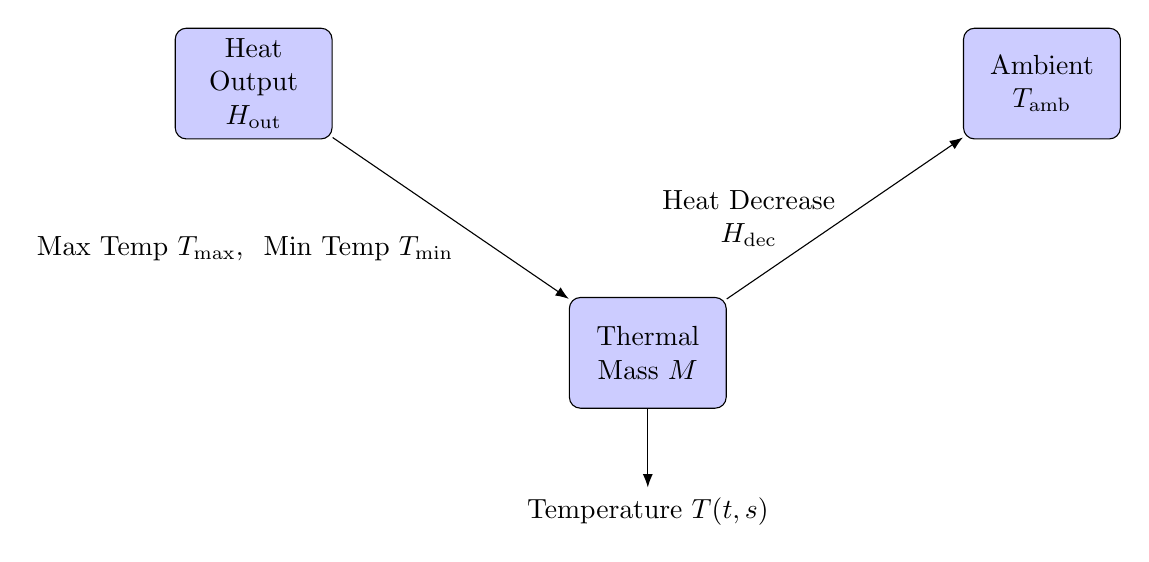
\begin{tikzpicture}[
    block/.style={rectangle, draw, fill=blue!20, text width=5em, text centered, rounded corners, minimum height=4em},
    line/.style={draw, -Latex},
    node distance=2cm and 3cm
]

% Nodes
\node[block] (thermalmass) {Thermal Mass $M$};
\node[block, above left=of thermalmass] (heater) {Heat Output\\$H_{\text{out}}$};
\node[block, above right=of thermalmass] (ambient) {Ambient $T_{\text{amb}}$};
\node[below=1cm of thermalmass] (temp) {Temperature $T(t,s)$};

% Paths
\path[line] (heater) -- node[anchor=south, midway, align=center] {} (thermalmass);
\path[line] (thermalmass) -- node[anchor=east, midway, align=center] {Heat Decrease\\$H_{\text{dec}}$} (ambient);
\path[line] (thermalmass) -- node[anchor=east] {} (temp);

% Constants
\node[below left=0.5cm and -1cm of heater, align=left] (maxtemp) {\\\\Max Temp $T_{\text{max}}$, };
\node[below right=0.5cm and -1cm of heater, align=right] (mintemp) {\\\\Min Temp $T_{\text{min}}$};

\end{tikzpicture}
\caption{Diagram of the Smart Home Heating System}
\end{figure}

Consider a smart home heating system designed to regulate the temperature of a house automatically. The system is meant to maintain indoor comfort based on the external temperature fluctuations and user-set temperature limits. Your task is to formalize the operation of this system using temporal situation calculus. Consider all temperatures in Celsius. \\
\\
The heat output can be controlled based on predefined temperature thresholds with actions $turnOnHeater(t)$ and $turnOffHeater(t)$. These action instantaneously change the fluent $heating(s)$ process. Let the temporal functional fluent $temp(t, s)$ represent the temperature of the home at time $t$. The system allows for a constant heat output $H_{\text{out}}$ (per unit time) when the heater is on and a constant heat decrease rate $H_{\text{dec}}$ (per unit time), influenced (multiplicatively) by the home's thermal mass $M$ and constant ambient temperature $T_{\text{amb}}$. The system is controlled to only change depending on a minimum $T_{\text{min}}$ and a maximum $T_{\text{max}}$ (i.e., you can only start heating if below $T_{\text{min}}$, or stop heating if above $T_{\text{max}}$, this is inversely true for venting) while also respecting the physical laws of thermodynamics, such as not allowing the temperature to drop below absolute zero (-273.15). Additionally, the system features a ventilation system which can cool the house more rapidly if needed. With actions $openVent(t)$ and $closeVent(t)$ the fluent $venting(s)$ process is instantaneously changed. When venting, the rate of $H_{\text{dec}}$ is doubled. Assume the temperature gain while heating is always more than ambient heat loss in the system. If the system is venting and heating, the temperature does not change.
\subsubsection*{Grading rubric:}
\\\\
{\textbf{(10\%)}} Define the \textbf{preconditions for the actions} $turnOnHeater(t)$, $turnOffHeater(t)$, $openVent(t)$, $closeVent(t)$. Consider under what conditions these actions are possible based on the system's current state and the time of action.\\
\\
{\textbf{(10\%)}} Define the \textbf{Successor State Axioms} for the fluents $heating(s)$ and $venting(s)$ process. These axioms should account for the changes in the state of these fluents based on the actions taken.\\
\\
{\textbf{(30\%)}} Specify how the \textbf{temporal fluent $temp$ should be initialized} following any action. Assume that there are no leaks in the system, meaning that temperature changes only occur due to the actions specified and the natural processes modeled.\\
\\
{\textbf{(50\%)}} \textbf{Develop a State Evolution Axiom} for $temp(t, s)$ that considers whether the heating or ventilation systems are active, and includes conditions for their influence on temperature over time. Also, incorporate the physical constraint on temperature.\\
\\
\subsubsection*{Instructions:}
Your answers should be logical formulas that clearly define how the smart home heating system operates according to the given constraints and actions. This exercise tests your understanding of situation calculus in designing complex system controls with multiple interacting components.

\subsection*{Solution:}

\subsubsection*{Precondition Axioms with Temporal Constraints:}
\begin{align*}
Poss(turnOnHeater(t), s) & \leftrightarrow \neg heating(s) \land t \geq start(s) \land (temp(t, s) < T_{\text{min}}). \\
Poss(turnOffHeater(t), s) & \leftrightarrow heating(s) \land t \geq start(s) \land (temp(t, s) > T_{\text{max}}). \\
Poss(openVent(t), s) & \leftrightarrow \neg venting(s) \land t \geq start(s) \land (temp(t, s) > T_{\text{max}}). \\
Poss(closeVent(t), s) & \leftrightarrow venting(s) \land t \geq start(s) \land (temp(t, s) < T_{\text{min}}). \\
\end{align*}

\subsubsection*{SSAs for Atemporal Fluents:}
\begin{align*}
heating(do(a, s)) & \leftrightarrow \exists t (a = turnOnHeater(t) \land \neg heating(s) \land temp(time(a), s) < T_{\text{min}}) \lor \\
                   & \phantom{\leftrightarrow \ } (heating(s) \land \neg \exists t (a = turnOffHeater(t) \land temp(time(a), s) > T_{\text{max}})).\\
venting(do(a, s)) & \leftrightarrow \exists t (a = openVent(t) \land \neg venting(s) \land temp(time(a), s) > T_{\text{max}}) \lor \\
                   & \phantom{\leftrightarrow \ } (venting(s) \land \neg \exists t (a = closeVent(t) \land temp(time(a), s) < T_{\text{min}})).                   
\end{align*}

\subsubsection*{SSAs to Initialize Temporal Fluents}
Initial value SSA for temperature:
\[
temp_{init}(do(a, s)) = T \leftrightarrow temp(time(a), s) = T.
\]

\subsubsection*{State Evolution Axiom (SEA) for Temperature}
\begin{align*}
temp(t, s) = T \leftrightarrow & \ \exists T_0 \exists t_0 \Big(temp_{init}(s) = T_0 \land start(s) = t_0 \land \\
& \Big( (heating(s) \land \neg venting(s) \land T = T_0 + H_{\text{out}} \cdot (t - t_0) - H_{\text{dec}} \cdot M \cdot T_{\text{amb}} \cdot (t - t_0)) \lor \\
& (\neg heating(s) \land venting(s) \land T = max\{T_0 - 2\cdot H_{\text{dec}} \cdot M \cdot T_{\text{amb}} \cdot (t - t_0), -273.15\})\lor\\
& ( heating(s) \land venting(s) \land T = T_0)\lor\\
& (\neg heating(s) \land \neg venting(s) \land  T = max\{T_0 - H_{\text{dec}} \cdot M \cdot T_{\text{amb}} \cdot (t - t_0), -273.15\})\Big)
\end{align*}

\end{problem}


\begin{problem}

\section*{New Evaluation 2: Assignment -- Forgetting and Progression}

\subsection*{Goal of the Assignment}
The primary goal of this assignment is to apply progression to a new domain within a software management system.

\section*{Steps to Solution}
To arrive at the solution for this assignment, students should:
\begin{enumerate}
    \item Model the system by defining the initial state and the fluents (conditions) involved.
    \item Analyze the preconditions and effects of the \texttt{updateSoftware} action within the system.
    \item Apply Successor State Axioms (SSAs) to derive the state of the system post-action execution.
    \item Identify which fluents are affected locally and globally by the action to understand its scope and impact.
    \item Transform the SSAs to reflect changes based on the specific actions taken and the initial system state.
    \item Define and utilize argument and characteristic sets for each relevant fluent to effectively model the system's progression.
    \item Implement the technique of forgetting and progression to multiple fluents.
\end{enumerate}

\subsection*{Assignment:}
Considers a computer system with various software components that can be updated. We address fluents that indicate the situation in terms of updates, vulnerabilities, and restart requirements.

\subsubsection*{Fluents}
\begin{itemize}
    \item $\texttt{updated}(component, s)$: True if a software component is updated in situation $s$.
    \item $\texttt{vulnerable}(component, s)$: True if a software component is vulnerable in situation $s$.
    \item $\texttt{requiresRestart}(system, s)$: True if the system requires a restart to apply updates in situation $s$.
\end{itemize}
\\
The initial state $S_0$ is defined as follows:
\[
\texttt{updated}(os, S_0) \land \neg \texttt{updated}(av, S_0) \land \texttt{vulnerable}(av, S_0) \land \neg \texttt{requiresRestart}(sys, S_0)
\]
Implicit types $\texttt{software(os)}$ and $\texttt{software(av)}$ are assumed for the operating system (os) and antivirus (av).\\
\\
Consider the following action:\\
\textbf{updateSoftware}$(component)$: Action to update a specific software component.
\begin{itemize}
    \item \textbf{Precondition:}
    \[
    \texttt{poss}(\texttt{do}(\texttt{updateSoftware}(c), s)) \leftrightarrow \texttt{software}(c) \land \texttt{vulnerable}(c, s)
    \]
    \item \textbf{Effect:}
    \[
    \texttt{updated}(c, \texttt{do}(\texttt{updateSoftware}(c), s))
    \]
    \[
    \texttt{requiresRestart}(sys, \texttt{do}(\texttt{updateSoftware}(c), s))
    \]
\end{itemize}

\subsubsection*{Successor State Axioms (SSAs)}
\begin{align*}
\texttt{updated}(c, \texttt{do}(a, s)) &\leftrightarrow \texttt{software}(c) \land \texttt{vulnerable}(c, s) \land a = \texttt{updateSoftware}(c) \lor \texttt{updated}(c, s) \\
&\land \neg(a=\texttt{injectVirus}(c) \lor (\exists sys).a=\texttt{restart}(sys)) \\
\texttt{vulnerable}(c, \texttt{do}(a, s)) &\leftrightarrow a=\texttt{injectVirus(c)}\lor \texttt{vulnerable}(c, s) \land \neg (a = \texttt{updateSoftware}(c))  \\
\texttt{requiresRestart}(sys, \texttt{do}(a, s)) &\leftrightarrow (\exists c). a = \texttt{updateSoftware}(c) \lor \texttt{requiresRestart}(sys, s) \land \neg(a=\texttt{restart}(sys))
\end{align*}
\\
Suppose the next situation is  $S_\alpha = \texttt{do}(\texttt{updateSoftware}(av), S_0)$. We would like to compute progression of the initial theory.

\subsubsection*{Assignment questions:}
\\\\
\begin{enumerate}
    \item {\textbf{(5\%)}} Identify which fluents are local effect wrt. updateSoftware(c).\\
\item {\textbf{(10\%)}} Derive transformed SSAs.\\
\item {\textbf{(15\%)}} Define the argument set $\Delta_F_j$ for each relevant fluent $F_j$. Generate the characteristic set $\Omega$ of $\alpha$, yeilding $\Omega(S_0)$.\\
\item {\textbf{(30\%)}} Instantiate SSA of $F_j$ on LHS with constants from $\Delta F_j$, combine SSAs yeilding $D_{ss}[\Omega]$ representing new values of the fluents.\\
\item {\textbf{(40\%)}} Forgetting and Progression: Let $\phi$ be $D_{S_0} \land D_{ss}[\Omega]$. The progression $D_{S_\alpha}$ is forget($\phi, \Omega(S_0)$), then replace $S_0$ with $S_\alpha$.\\
\end{enumerate}
Let $\top$ and $\bot$ be a new propositional constant as an abbreviation for $(S_0=S_0)$ and $\neg(S_0=S_0)$, True and False respectively.

\subsection*{Solution:}

\subsubsection*{Q1: Identify which fluents are local effect wrt. updateSoftware(c).}

Local effect:
\begin{itemize}
    \item updated(c,s) -- updateSoftware(c) has local effect on fluent updated since all object arguments are included.
    \item vulnerable(c,s) -- updateSoftware(c) has local effect on fluent vulnerable since all object arguments are included.
\end{itemize}
\\\\
Global effect:
\begin{itemize}
    \item requiresRestart(sys,s) -- updateSoftware(c) has global effect on fluent requiresRestart since the action has at least one universally-quantified object argument not included.
\end{itemize}

\subsubsection*{Q2: Derive transformed SSAs.}
Updated SSA transformation:
\begin{align*}
&\texttt{updated}(c, \texttt{do}(\texttt{updateSoftware}(av), S_0)) \leftrightarrow &\\
&\texttt{software}(c) \land \texttt{vulnerable}(c, S_0) \land \texttt{updateSoftware}(av) = \texttt{updateSoftware}(c) \lor \texttt{updated}(c, S_0) &\\
&\land \neg(\texttt{updateSoftware}(av)=\texttt{injectVirus}(c) \lor (\exists sys).\texttt{updateSoftware}(av)=\texttt{restart}(sys)) &\\\\
\equiv&\texttt{updated}(c, \texttt{do}(\texttt{updateSoftware}(av), S_0)) \leftrightarrow \texttt{software}(c) \land \texttt{vulnerable}(c, S_0) \land av = c \lor \texttt{updated}(c, S_0) \land \neg(\bot \lor \bot) &\tag{UNA \& Simplify}\\
\equiv&\texttt{updated}(c, \texttt{do}(\texttt{updateSoftware}(av), S_0)) \leftrightarrow \texttt{software}(c) \land \texttt{vulnerable}(c, S_0) \land av = c \lor \texttt{updated}(c, S_0) &\tag{Simplify}
\end{align*}
\\
Vulnerable SSA transformation:
\begin{align*}
&\texttt{vulnerable}(c, \texttt{do}(\texttt{updateSoftware}(av), S_0)) \leftrightarrow \texttt{updateSoftware}(av)=\texttt{injectVirus(c)}\lor \texttt{vulnerable}(c, S_0) &\\
&\land \neg (\texttt{updateSoftware}(av) = \texttt{updateSoftware}(c)) & \\\\
\equiv&\texttt{vulnerable}(c, \texttt{do}(\texttt{updateSoftware}(av), S_0)) \leftrightarrow \bot \lor \texttt{vulnerable}(c, S_0) \land \neg (av = c) & \tag{UNA \& Simplify}\\
\equiv&\texttt{vulnerable}(c, \texttt{do}(\texttt{updateSoftware}(av), S_0)) \leftrightarrow \texttt{vulnerable}(c, S_0) \land \neg (av = c) & \tag{Simplify}
\end{align*}
\\
requiresRestart SSA transformation:
\begin{align*}
& \texttt{requiresRestart}(sys, \texttt{do}(\texttt{updateSoftware}(av), S_0)) \leftrightarrow (\exists c). \texttt{updateSoftware}(av) = \texttt{updateSoftware}(c) &\\
&\lor \texttt{requiresRestart}(sys, S_0) \land \neg(\texttt{updateSoftware}(av)=\texttt{restart}(sys))&\\\\
\equiv& \texttt{requiresRestart}(sys, \texttt{do}(\texttt{updateSoftware}(av), S_0)) \leftrightarrow (\exists c). av = c \lor \texttt{requiresRestart}(sys, S_0) \land \neg(\bot)&\tag{UNA \& Simplify}\\
\equiv& \texttt{requiresRestart}(sys, \texttt{do}(\texttt{updateSoftware}(av), S_0)) \leftrightarrow (\exists c). av = c \lor \texttt{requiresRestart}(sys, S_0) &\tag{Simplify}\\
\equiv& \texttt{requiresRestart}(sys, \texttt{do}(\texttt{updateSoftware}(av), S_0)) \leftrightarrow \top \lor \texttt{requiresRestart}(sys, S_0) &\tag{By BAT}\\
\equiv& \texttt{requiresRestart}(sys, \texttt{do}(\texttt{updateSoftware}(av), S_0)) \leftrightarrow \top &\tag{Simplify}\\
\end{align*}

\subsubsection*{Q3:  Define the argument set $\Delta_F_j$ for each relevant fluent $F_j$. Generate the characteristic set $\Omega$ of $\alpha$.}

Argument sets:
\[\Delta_{updated}=\{av\}\]
\[\Delta_{vulnerable}=\{av\}\]
\\\\
Characteristic set:
\[\Omega(S_0) = \{\texttt{vulnerable}(av, S_0), \texttt{updated}(av, S_0)\}\]
These should be forgotten. 

\subsubsection*{Q4: Instantiate SSA of $F_j$ on LHS with constants from $\Delta F_j$, combine SSAs yeilding $D_{ss}[\Omega]$ representing new fluent values.}
Instantiate updated SSA:
\begin{align*}
&\texttt{updated}(av, \texttt{do}(\texttt{updateSoftware}(av), S_0)) \leftrightarrow \texttt{software}(av) \land \texttt{vulnerable}(av, S_0) \land av = av \lor \texttt{updated}(av, S_0) &\\
\equiv&\texttt{updated}(av, \texttt{do}(\texttt{updateSoftware}(av), S_0)) \leftrightarrow \texttt{software}(av) \land \texttt{vulnerable}(av, S_0) \lor \texttt{updated}(av, S_0) &\tag{Simplify $\top$}\\
\equiv&\texttt{updated}(av, \texttt{do}(\texttt{updateSoftware}(av), S_0)) \leftrightarrow \top \land \top \lor \bot &\tag{By $S_0$}\\
\equiv&\texttt{updated}(av, \texttt{do}(\texttt{updateSoftware}(av), S_0))&
\end{align*}
\\
Instantiate vulnerable SSA:
\begin{align*}
&\texttt{vulnerable}(av, \texttt{do}(\texttt{updateSoftware}(av), S_0)) \leftrightarrow \texttt{vulnerable}(av, S_0) \land \neg (av = av) & \\
\equiv&\texttt{vulnerable}(av, \texttt{do}(\texttt{updateSoftware}(av), S_0)) \leftrightarrow \texttt{vulnerable}(av, S_0) \land \neg (\top) & \\
\equiv&\neg\texttt{vulnerable}(av, \texttt{do}(\texttt{updateSoftware}(av), S_0))  & 
\end{align*}

\[D_{ss}[\Omega] = \{\texttt{updated}(av, \texttt{do}(\texttt{updateSoftware}(av), S_0)), \neg\texttt{vulnerable}(av, \texttt{do}(\texttt{updateSoftware}(av), S_0))\}\]

\subsubsection*{Q5: Forgetting and Progression}

Let $\phi$ be $D_{S_0} \land D_{ss}[\Omega]$. The progression $D_{S_\alpha}$ is forget($\phi, \Omega(S_0)$), then replace $S_0$ with $S_\alpha$.\\
\[\phi\equiv(\texttt{updated}(os, S_0) \land \neg \texttt{updated}(av, S_0) \land \texttt{vulnerable}(av, S_0) \land \neg \texttt{requiresRestart}(sys, S_0)) \lor \]
\[(\texttt{updated}(av, \texttt{do}(\texttt{updateSoftware}(av), S_0))\land \neg\texttt{vulnerable}(av, \texttt{do}(\texttt{updateSoftware}(av), S_0)))\]
\\
\\
The forget replacements for vulnerable and updated fluents:
\[\phi[\texttt{vulnerable}] = x=av \land y=S_0 \land \texttt{vulnerable}(av, S_0) \lor \neg(x=av \land y=S_0) \land \texttt{vulnerable}(x, y)\]
\[\phi[\texttt{updated}] = x=av\land y=S_0\land \texttt{updated}(av, S_0) \lor \neg(x=av\land y=S_0)\land \texttt{updated}(x, y)\]
\\
Forgetting two different fluents sequentially. \\
\\
Forget vulnerable first:
\[\texttt{forget}(\phi, \texttt{vulnerable}) = \phi^{+}\lor\phi^-\]
\(\phi^+\equiv(\texttt{updated}(os, S_0) \land \neg \texttt{updated}(av, S_0) \land (av=av \land S_0=S_0 \land \texttt{vulnerable}(av, S_0) \lor \neg(av=av \land S_0=S_0) \land   \)\\
\(\texttt{vulnerable}(av, S_0)) \land\neg \texttt{requiresRestart}(sys, S_0)) \lor(\texttt{updated}(av, \texttt{do}(\texttt{updateSoftware}(av), S_0))\land \neg(av=av \land\)\\
\(  \texttt{do}(\texttt{updateSoftware}(av), S_0)=S_0 \land \texttt{vulnerable}(av, S_0) \lor \neg(av=av \land \texttt{do}(\texttt{updateSoftware}(av), S_0)=S_0) \)\\
\(\land \texttt{vulnerable}(av, \texttt{do}(\texttt{updateSoftware}(av), S_0)))\)\\
\\
\(\phi^+\equiv(\texttt{updated}(os, S_0) \land \neg \texttt{updated}(av, S_0) \land (\top \land \top \land \texttt{vulnerable}(av, S_0) \lor \neg(\top \land \top) \land  \texttt{vulnerable}(av, S_0)) \land \)\\
\(\neg \texttt{requiresRestart}(sys, S_0)) \lor(\texttt{updated}(av, \texttt{do}(\texttt{updateSoftware}(av), S_0))\land \neg(\top \land \bot \land \texttt{vulnerable}(av, S_0) \lor\)\\
\(  \neg(\top \land \bot) \land \texttt{vulnerable}(av, \texttt{do}(\texttt{updateSoftware}(av), S_0)))\)\\
\\
\(\phi^+\equiv(\texttt{updated}(os, S_0) \land \neg \texttt{updated}(av, S_0) \land  \neg \texttt{requiresRestart}(sys, S_0) \lor\)\\
\((\texttt{updated}(av, \texttt{do}(\texttt{updateSoftware}(av), S_0))\land \neg\texttt{vulnerable}(av, \texttt{do}(\texttt{updateSoftware}(av), S_0)))\)\\
\\
\(\phi^+\equiv(\texttt{updated}(av, \texttt{do}(\texttt{updateSoftware}(av), S_0))\land \neg\texttt{vulnerable}(av, \texttt{do}(\texttt{updateSoftware}(av), S_0)))\)\\
\\
Now, interpret $\texttt{vulnerable}(av, S_0)$ as false:\\
\(\phi^-\equiv(\texttt{updated}(os, S_0) \land \neg \texttt{updated}(av, S_0) \land (\texttt{vulnerable}(av, S_0)  \land  \neg \texttt{requiresRestart}(sys, S_0)) \lor\)\\
\((\texttt{updated}(av, \texttt{do}(\texttt{updateSoftware}(av), S_0))\land \neg\texttt{vulnerable}(av, \texttt{do}(\texttt{updateSoftware}(av), S_0)))\)\\
\\
\(\phi^-\equiv\texttt{updated}(av, \texttt{do}(\texttt{updateSoftware}(av), S_0))\land \neg\texttt{vulnerable}(av, \texttt{do}(\texttt{updateSoftware}(av), S_0))\)\\
\\
Therefore, \\
\(\texttt{forget}(\phi, \texttt{vulnerable}) =\)
\[ \texttt{updated}(av, \texttt{do}(\texttt{updateSoftware}(av), S_0))\land \neg\texttt{vulnerable}(av, \texttt{do}(\texttt{updateSoftware}(av), S_0))\]
\\
\begin{theorem}[LiuLakemeyer2009, Theorem 2.4]
Let \( G \) be a finite set of ground atoms and \( \phi \) a formula. Then, \( \text{forget}(\phi, G) \) and \( \bigvee_{A \in \mathcal{M}(G)} \phi^{A} \) are logically equivalent.
\end{theorem}
\\
% Explanation text
Forgetting about a set \( G \) of ground literals amounts to forgetting about each literal one after another, i.e., if \( G = \{P_1, \ldots, P_n\} \), then \( \text{forget}(\phi, G) = \text{forget}(\ldots\text{forget}(\text{forget}(\phi, P_1), P_2)\ldots, P_n) \).
\\
\\
Therefore by (LiuLakemeyer2009, Theorem 2.4) we now forget update sequentially using $\phi[\texttt{updated}]$:\\
\\
\(\texttt{forget}(\texttt{forget}(\phi, \texttt{vulnerable}), \texttt{update}) \equiv \phi^+ \lor \phi^-\)\\
\\
\(\phi^+\equiv(av=av\land \texttt{do}(\texttt{updateSoftware}(av), S_0)=S_0\land \texttt{updated}(av, S_0) \lor \)\\
\(\neg(av=av\land \texttt{do}(\texttt{updateSoftware}(av), S_0)=S_0)\land \texttt{updated}(av, \texttt{do}(\texttt{updateSoftware}(av), S_0))) \land \)\\
\(\neg\texttt{vulnerable}(av, \texttt{do}(\texttt{updateSoftware}(av), S_0))\)\\
\\
\(\phi^+\equiv (\top\land \bot \land \top \lor \neg(\top\land \bot)\land \texttt{updated}(av, \texttt{do}(\texttt{updateSoftware}(av), S_0))) \land  \neg\texttt{vulnerable}(av, \texttt{do}(\texttt{updateSoftware}(av), S_0))\)
\\
\(\phi^+ \equiv \texttt{updated}(av, \texttt{do}(\texttt{updateSoftware}(av), S_0)) \land  \neg\texttt{vulnerable}(av, \texttt{do}(\texttt{updateSoftware}(av), S_0))\)\\
\\
\\
\(\phi^-\equiv(av=av\land \texttt{do}(\texttt{updateSoftware}(av), S_0)=S_0\land \texttt{updated}(av, S_0) \lor \)\\
\(\neg(av=av\land \texttt{do}(\texttt{updateSoftware}(av), S_0)=S_0)\land \texttt{updated}(av, \texttt{do}(\texttt{updateSoftware}(av), S_0))) \land \)\\
\(\neg\texttt{vulnerable}(av, \texttt{do}(\texttt{updateSoftware}(av), S_0))\)\\
\\
\(\phi^-\equiv(\top\land \bot\land \bot \lor \neg(\top\land \bot)\land \texttt{updated}(av, \texttt{do}(\texttt{updateSoftware}(av), S_0))) \land \neg\texttt{vulnerable}(av, \texttt{do}(\texttt{updateSoftware}(av), S_0))\)\\
\\
\(\phi^-\equiv\texttt{updated}(av, \texttt{do}(\texttt{updateSoftware}(av), S_0)) \land \neg\texttt{vulnerable}(av, \texttt{do}(\texttt{updateSoftware}(av), S_0))\)\\
\\
Therefore, \\
\(\texttt{forget}(\texttt{forget}(\phi, \texttt{vulnerable}), \texttt{update})  =\texttt{forget}(\phi, \Omega(S_0))=\)
\[ \texttt{updated}(av, \texttt{do}(\texttt{updateSoftware}(av), S_0)) \land \neg\texttt{vulnerable}(av, \texttt{do}(\texttt{updateSoftware}(av), S_0))\]
\\
Finally, we replace $S_0$ with $S_\alpha$ to arrive at $D_{S_\alpha}$: \\
\[D_{S_\alpha}\equiv \texttt{updated}(av, \texttt{do}(\texttt{updateSoftware}(av), S_\alpha)) \land \neg\texttt{vulnerable}(av, \texttt{do}(\texttt{updateSoftware}(av), S_\alpha))\]
This completes the progression.
\end{problem}
\\
\section*{References:}\\
Soutchanski, Mikhail. CPS822 Lectures \& Notes, 2024, Toronto Metropolitan University, Toronto, ON.\\

\hline
\hline
\text{}\\
\noindent $\square$	In working on and submitting this evaluation, I pledge to adhere to Policy 60 and 
the framework for the evaluation as specified by my instructor, and as mentioned in 
the CPS822 Course Management Form. The work submitted is my own work.  I have not consulted 
with other people. I cited explicitly all external sources, if any.
\end{document}




% \section*{Example 2: a Water Reservoir}

% \begin{tabular}{ccc}
% inflow rate $R_{\text{in}}$ & water volume $V$ & max volume = tank capacity $C$ \\
%  & $\updownarrow$ & min volume = 0 \\
%  & outflow rate $R_{\text{out}}$ & \\
% \end{tabular}

% Consider a water reservoir with an adjustable inflow and an adjustable outflow. Let the temporal functional fluent $vol(t, s)$ represent the volume of water in the tank at time $t$. The maximum capacity of the tank is $C$. Let $R_{\text{in}}$ and $R_{\text{out}}$ be inflow and outflow rates (volume per unit time), which are for simplicity are constant, i.e., rates are time-invariant.

% Let actions $startIn(t)$, $endIn(t)$ represent opening/closing of the inflow valve. These actions initiate/terminate the process represented as the fluent $inflow(s)$. Let actions $startOut(t)$, $endOut(t)$ represent opening/closing of the outflow valve. These actions initiate/terminate the process outflow$(s)$.

% \subsection*{Precondition Axioms with Temporal Constraints:}
% \begin{align*}
% Poss(startIn(t), s) & \leftrightarrow inflow(s) \land t \geq start(s) \land (vol(t, s) < C). \\
% Poss(endIn(t), s) & \leftrightarrow inflow(s) \land t \geq start(s). \\
% Poss(startOut(t), s) & \leftrightarrow \neg outflow(s) \land t \geq start(s) \land (vol(t, s) > 0). \\
% Poss(endOut(t), s) & \leftrightarrow outflow(s) \land t \geq start(s). \\
% \end{align*}

% \subsection*{SSAs for Atemporal Fluents:}
% \begin{align*}
% inflow(do(a, s)) & \leftrightarrow \exists t (a = startIn(t)) \land inflow(s) \land \neg \exists t (a = endIn(t)) \\
% outflow(do(a, s)) & \leftrightarrow \exists t (a = startOut(t)) \land outflow(s) \land \neg \exists t (a = endOut(t)) \\
% \end{align*}
% \section*{SSAs to Initialize Temporal Fluents}
% An obvious initial value SSA asserts the continuity of volume (no leaks):
% \[
% vol_{init}(do(a, s)) = v \leftrightarrow vol(time(a), s) = v.
% \]
% \section*{Reservoir: a State Evolution Axiom (SEA) for Volume}
% To write a State Evolution Axiom for the fluent $vol(t, s)$ consider all possible combinations of inflow and outflow: either the inflow valve is open while outflow is present or not, or the inflow valve is closed while the outflow valve can be open or closed. Each combination is a separate context. For each context, $vol(t, s)$ evolves according to a different function of flow rates and time. Inflow cannot exceed capacity $C$, and outflow cannot yield $vol(t, s) < 0$.

% \begin{align*}
% vol(t, s) = v \leftrightarrow & \ \exists t_0 \Big(vol_{init}(s) = v_0 \land start(s) = t_0 \land \\
% & \big((inflow(s) \land \neg outflow(s)) \land v = min\{v_0 + R_{\text{in}} \cdot (t - t_0), C\} \lor \\
% & (inflow(s) \land outflow(s)) \land v = max\{min\{v_0 + R_{\text{in}} \cdot (t - t_0) - R_{\text{out}} \cdot (t - t_0), C\}, 0\} \lor \\
% & (\neg inflow(s) \land outflow(s)) \land v = max\{v_0 - R_{\text{out}} \cdot (t - t_0), 0\} \lor \\
% & (\neg inflow(s) \land \neg outflow(s)) \land v = v_0 \Big).
% \end{align*}

% The expression $\neg inflow(s) \land \neg outflow(s)$ on the last line of the SEA is logically equivalent to the negated disjunction of the three contexts on the preceding lines. Notice that in this axiom there are four different pairwise exclusive contexts, and for each context there is its own function describing how the fluent evolves with time.


% \subsection*{Solution:}

% \subsection*{Rubric:}


% \noindent








% Consider a kitchen domain where there are fluents \texttt{washed}(\textit{item}), \texttt{seasoned}(\textit{meat}), \texttt{heated}(\textit{stove}) with the self-evident SSAs. Also, there is \texttt{cooked}(\textit{i}, \textit{s}) meaning that the item \textit{i} is cooked in situation \textit{s}. Let the initial theory be $\texttt{washed}(V_1, S_0)\land \texttt{washed}(V_2, S_0)\land \texttt{seasoned}(M, S_0)\land \texttt{heated}(SV, S_0) \land \neg \texttt{cooked}(M,S_0)\land \neg \texttt{cooked}(V_2,S_0)$ and the implicit types \texttt{stove}(\(SV\)) $\land$ \texttt{meat}(\(M\)) $\land$ \texttt{vegetable}(\(V_2\)) are omitted, for brevity.

% Consider an action \texttt{cookTogether}(\(m, v, sv\)): cook a meat \(m\) and a vegetable \(v\) together on the stove \(sv\). Suppose the next situation is \(S_\alpha = \texttt{do}(\texttt{cookTogether}(\(M, V_2, SV\)), S_0)\). We would like to compute progression of the initial theory.

% Precondition axiom:
% \[
% \forall sv\forall m \forall v \forall s. \texttt{poss}(\texttt{cookTogether}(m, v, sv), s) \leftrightarrow \]
% \[\texttt{stove}(sv) \land \texttt{meat}(m) \land \texttt{heated}(sv, s) \land \texttt{seasoned}(m, s) \land \texttt{washed}(v, s) \land \lnot(\texttt{cooked}(m, s) \lor \texttt{cooked}(v, s))
% \]

% This action has a positive effect on the fluent \texttt{cooked}(\textit{item}, \textit{s}) with the SSA 
% \[
% \forall i, a, s. \texttt{cooked}(i, \texttt{do}(a, s)) \leftrightarrow \]
% \[\Big(\texttt{vegetable}(i) \land \exists sv(a=\texttt{cookVegetable}(i, sv) \lor \exists m(m=a=\texttt{cookTogether}(m, i, sv)))\Big)\]
% \[ \lor \Big(\texttt{meat}(i) \land \exists sv(a=\texttt{cookMeat}(i, sv) \lor \exists v(a=\texttt{cookTogether}(i, v, sv)))\Big) \lor \texttt{cooked} (i,s)
% \]

% To trace progression algorithm, follow the steps from the handout. (1) Start with writing \textit{transformed} SSAs. Replace action variable with the ground action \(\alpha\) and then do logically equivalent simplifications.

% \textbf{Unchanged}(\(x\)):
% \[
% \forall v \forall s. \texttt{washed}(v, \texttt{do}(\texttt{cookTogether}(M, V_2, SV), s)) \leftrightarrow \texttt{washed}(v, s)
% \]
% \[
% \forall m, s. \texttt{seasoned}(m, \texttt{do}(\texttt{cookTogether}(M, V_2, SV), s)) \leftrightarrow \texttt{seasoned}(m, s)
% \]
% \[
% \forall sv, v, s. \texttt{heated}(sv, \texttt{do}(\texttt{cookTogether}(M, V_2, SV), s)) \leftrightarrow \texttt{heated}(sv, s)
% \]

% To trace progression algorithm, follow the steps from the handout. (1) Start with writing \textit{transformed SSAs}. Replace action variable with the ground action a and then do logically equivalent simplifications.

% \begin{align*}
% \forall v\forall s.\ \textit{washed}(v, \text{do}(\text{cookTogether}(M, V_2, SV), s)) &\iff \textit{washed}(v, s) \\
% \forall m, s.\ \textit{seasoned}(m, \text{do}(\text{cookTogether}(M, V_2, SV), s)) &\iff \textit{seasoned}(m, s) \\
% \forall sv, v, s.\ \textit{heated}(sv, \text{do}(\text{cookTogether}(M, V_2, SV), s)) &\iff \textit{heated}(sv, s) \\\\
% \forall i, s.\ \textit{cooked}(i, \text{do}(\text{cookTogether}(M, V_2, s), s)) &\iff 
% \end{align*}
% \[ \left(\textit{vegetable}(i) \land \exists sv(\text{cookTogether}(M, V_2, SV) = \text{cookVegetable}(i, sv))\right) \lor \]
% \[ \left(\exists m(\text{cookTogether}(M, V_2, SV) = \text{cookTogether}(m, i, sv))) \land \textit{meat}(i) \land \exists sv(\text{cookTogether}(M, V_2, SV) = \text{cookMeat}(i, sv))\right) \lor \]
% \[ \left(\exists u(\text{cookTogether}(M, V_2, SV) = \text{cookTogether}(i, v, sv)) \land \textit{cooked}(i, s)\right) \]
% \begin{align*}
% &\equiv \left(\textit{vegetable}(i) \land \exists sv(\bot \land \exists m(m = M \land i = V_2 \land sv = SV))\right) \lor \\
% &\ \ \left(\textit{meat}(i) \land \exists sv(\bot \land \exists u(i = M \land v = V_2 \land sv = SV))\right) \lor \textit{cooked}(i, s) \\
% &\equiv \left(\textit{vegetable}(i) \land i = V_2 \land \exists m(m = M) \land \exists sv(sv = SV)\right) \lor \\
% &\ \ \left(\textit{meat}(i) \land i = M \land \exists sv(sv = SV)\right) \lor \textit{cooked}(i, s) \\
% &\equiv \left(\textit{vegetable}(i) \land i \neq V_2\right) \lor \left(\textit{meat}(i) \land i \neq M\right) \lor \textit{cooked}(i, s) \\
% \end{align*}

% (2) The argument set for the fluent \textit{cooked}(x, s) is $\Delta_{\textit{cooked}} = \{V_2, M\}$

% The characteristic set of all fluents subject to have their values change $\Omega(S_0) = \{\textit{cooked}(V_2, S_0), \textit{cooked}(M, S_0)\}$.

% They must be forgotten.